
\chapter{平台软件规划——连接确认(CC)}

 参考文件: Module Design of XX (Template).xlsx \cite{MDOT1};   
  
 \begin{enumerate}[label=\textbullet]
	\item  Introduce;
        \begin{enumerate}[label={}]
            \item \textcolor{red}{A brief description of the design module, which explains the functions that the modules needs to implement;}
        \end{enumerate}
	\item  Module Ports;
        \begin{enumerate}[label={}]
            \item \textcolor{red}{Don't need to write the specific ports, just write ``For more details about the modules ports, please refer to the related module interface files";}
        \end{enumerate}
	\item  Design Contents;
        \begin{enumerate}[label={}]
            \item \textcolor{red}{Before starting the design, the engineer should read the relevant information in ReadMe;}
        \end{enumerate}
\end{enumerate}

PP(Proximity Pilot)功能:PP 信号主要用于检测充电枪的物理状态,即充电插头的插
入深度和连接情况。PP 信号通过在插头和插座之间的物理连接来检测接近状态。作用:确认
充电枪是否插入到位。防止在插头未完全插入的情况下启动充电。确定充电电缆的额定电流
上限,以便限制通过充电线缆的最大电流,避免电缆过载。

CC(Connection Confirmation)功能:CC 信号负责最终确认连接的整体安全性,并在
充电开始前完成所有必要的检查。它通常依赖于 CP 和 PP 信号提供的信息,以确定是否可以
安全地开始充电。作用:确认 PP 信号的接近检测状态,以及 CP 信号的通信和控制状态。在
确认连接安全、无误后,允许充电电流传输。如果在充电过程中发现任何异常情况,CC 信号
将触发充电中断。

充电规范GB-T 18487.1-2015\cite{GB18487_1}:
    \begin{enumerate}
        \item 对于充电模式3,可以ABC三种连接方式,单相供电最大电流不超过16 A;
        \item 对于充电模式3,三相供电时电流大于32 A应采样连接方式C;
    \end{enumerate}

本文档适用于充电设备在{\bf 充电模式3 连接方式B}工作状态下的使用规范。

\section{Introduce}
 连接确认模块(Connect comfirm),在SAE\_J1772中是接近检测(Proximity Detection)\cite{SAE}。 
 这两个信号的关系不一致: PP $\longrightarrow$ CP $\longrightarrow$ CC。

 PP信号主要用于检测充电枪的物理状态,即充电插头的插入深度和连接情况。PP信号通过在插头和插座之间的物理连接来检测接近状态。
 \begin{enumerate}
    \item  确认充电枪是否插入到位;
    \item  防止在插头未完全插入的情况下启动充电;
    \item  确定充电电缆的额定电流上限,以便限制通过充电线缆的最大电流,避免电缆过载。
 \end{enumerate}

%  \begin{figure}[!htbp]
%     \centering
%     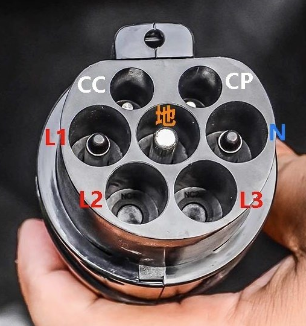
\includegraphics[width = 0.45\textwidth]{C3}
%     \caption{\href{https://www.chooseauto.com.cn/news/89436.shtml}{交流充电接口}}
%     \label{fig:C3}
% \end{figure}

\begin{figure}[!htbp]
    \centering
    \begin{subfigure}[b]{0.45\textwidth}
        \centering
        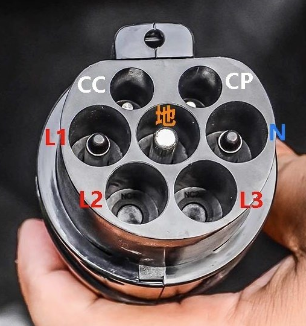
\includegraphics[width=0.65\textwidth]{C3} 
        \caption{交流充电接口}
        \label{fig:C3}
    \end{subfigure}
    \hspace*{-0.6cm}
    \begin{subfigure}[b]{0.45\textwidth}
        \centering
        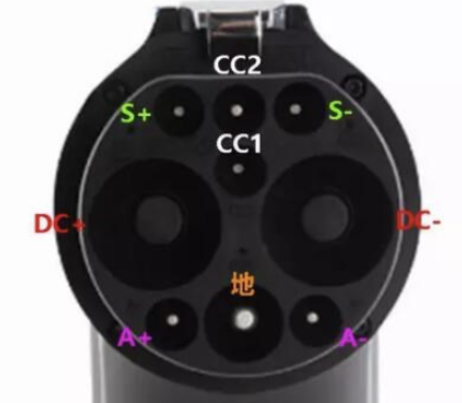
\includegraphics[width=0.8\textwidth]{C8} 
        \caption{直流充电接口}
        \label{fig:C8}
    \end{subfigure}
    \begin{subfigure}[b]{0.45\textwidth}
        \centering
        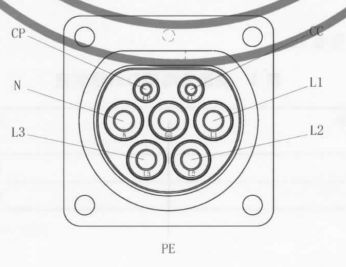
\includegraphics[width=0.8\textwidth]{C9} 
        \caption{交流充电接口\cite{GB20234_2}}
        \label{fig:C9}
    \end{subfigure}
    \hspace*{-0.6cm}
    \begin{subfigure}[b]{0.45\textwidth}
        \centering
        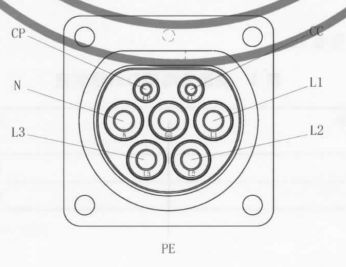
\includegraphics[width=0.8\textwidth]{C10} 
        \caption{直流充电接口\cite{GB20234_3}}
        \label{fig:C10}
    \end{subfigure}
    \caption{\href{https://www.chooseauto.com.cn/news/89436.shtml}{充电接口}}
    \label{fig:main}
\end{figure}



\begin{figure}[!htbp]
    \centering
    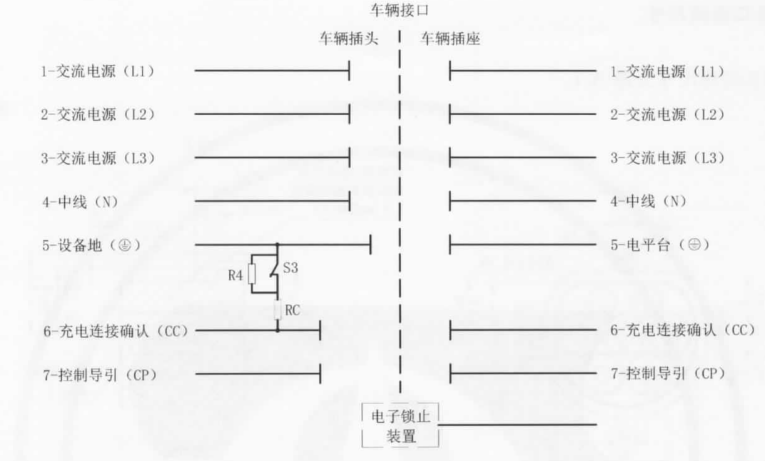
\includegraphics[width = 0.65\textwidth]{C5}
    \caption{车辆接口电气连接示意图}
    \label{fig:C5}
\end{figure}

\section{Modules Ports}


\section{Design Contents}

(1) 车辆控制装置测量检测点 2 有无 12 V CP 信号。如有
则标志着车辆插头与车辆插座已连接,控制导引电
路激活进入工作状态;如无,则控制导引电路处于
待机状态。%[8]。

(2) 车辆控制装置通过测量检测点 3 与
PE 之间的电阻值来判断车辆插头与车辆插座是否
完全连接。半连接时,S3 断开,检测点 3 与 PE 之
间的电阻为 RC+R4;完全连接时,S3 处于闭合状
态,检测点 3 与 PE 之间的电阻值为 RC。

(3) 供电控制装置通过测量检测点 1 的电压判断 R3 是否接
入,如 R3 接入则延时一定时间,将 S1 切换至 PWM输出状态。

(4) 车辆检测装置通过测量检测点 2 的
PWM 信号,判断充电装置是否已经完全连接。如
完全连接,则闭合开关 S2,车辆进入准备就绪状态。

(5) 供电控制装置通过进一步测量检测点 1 的电压
判断车辆是否进入准备就绪状态,如已进入就绪状
态,则闭合 K1、K2,交流供电回路导通。%[11]。

(6) 车辆控制装置通过测量检测点 2 的 PWM 信号占空比
确认供电设备的最大供电能力,并以此确定车载充
电机的输出电流,启动充电过程。%[9]。


\begin{figure}[!htbp]
    \centering
    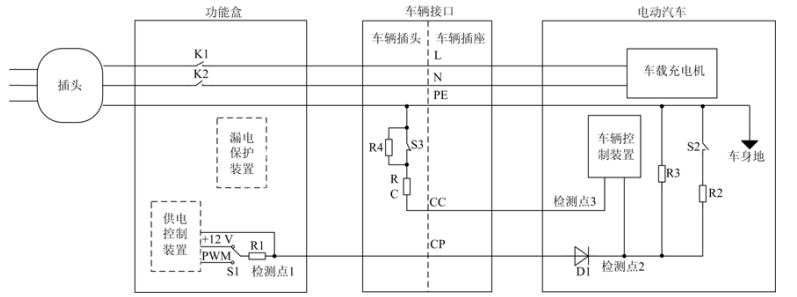
\includegraphics[width = 0.72\textwidth]{C4}
    \caption{交流充电模式2连接方式B}
    \label{fig:C3}
\end{figure}



\subsection{计算流程}
\subsubsection*{电流因子}
        计算电流的原始采样值:
            \begin{equation}
                \mathrm{Raw\_CC\_Current} = \mathrm{CC\_Current\_Factor} \times  \mathrm{ADC\_CC\_Current}
                \label{eq:CC1}
            \end{equation}

    \subsubsection*{一阶滤波}
        采样频率100 Hz,无延时;一阶传递函数表示如下:
            \begin{equation}
                G(s) = \frac{\omega_c}{s+\omega_c}
                \label{eq:CC2}
            \end{equation}
        或者:
            \begin{equation}
                G(s) = \frac{1}{T_cs+1}
                \label{eq:CC3}
            \end{equation}
        其中,$\omega_c$表示截止频率,$T_c$表示时间常数。离散化,后向差分,令$s = \frac{1-z^{-1}}{T_s}$, $T_s$表示采样周期。
        可以得到差分方程:
            \begin{equation}
                y(k) = \frac{\omega_cT_s}{1+\omega_cT_s}x(k)+\frac{1}{1+\omega_cT_s}y(k-1)
            \end{equation}
        令$a = \frac{\omega_cT_s}{1+\omega_cT_s}$, $1-a = \frac{1}{1+\omega_cT_s} $:
            \begin{equation}
                y(k) = ax(k)+(1-a)y(k-1)
                \label{eq:CC4}
            \end{equation}
        \textcolor{red}{CC\_Current滤波:}
            \begin{enumerate}[label={}]
                \item $y = \mathrm{Samp\_CC\_Current} $;
                \item $x = \mathrm{Raw\_CC\_Current} $;
                \item $a = \mathrm{CC\_Current\_FilterFactor}$
            \end{enumerate}
        系数$a$决定了滤波器的带宽:
            \begin{equation}
                \begin{cases}
                    \text{当 $a$ 较小时,滤波平稳,灵敏度低}\\
                    \text{当 $a$ 较大时,滤波毛刺大,灵敏度高}
                \end{cases}
            \end{equation}
    
   
        










\begin{algorithm} 
    \caption{连接确认(Connection Confirmation)} 
    \label{alg3} 
    \makebox[1\textwidth][c]{ % 设置宽度为文本宽度并居中
    \begin{minipage}{0.91\textwidth} % 设置算法宽度为 80% 文本宽度
    \renewcommand{\baselinestretch}{1.5} % 设置行距为 1.5 倍
    \selectfont
    \begin{algorithmic}[1] % [1] 表示显示行号
        \REQUIRE ADC\_CC\_Current, CC\_Current\_Limit$i$($i=1,2,3,4$);
        \ENSURE CCM\_CC\_Status, CCM\_CC\_MaxACCurent;
        \STATE 获取CC电流AD采样值:ADC\_CC\_Current;
        \STATE 1)计算CC原始采样电流:Raw\_CC\_Current,根据(\ref{eq:CC1});
        \STATE 2)计算CC滤波采样电流: Samp\_CC\_Current,根据(\ref{eq:CC4});
        \IF{$n < 0$} 
            \STATE $X \gets 1 / x$ 
            \STATE $N \gets -n$ 
        \ELSE 
            \STATE $X \gets x$ 
            \STATE $N \gets n$ 
        \ENDIF 
        \WHILE{$N \neq 0$} 
            \IF{$N$ 是偶数} 
                \STATE $X \gets X \times X$ 
                \STATE $N \gets N / 2$ 
            \ELSE 
                \STATE $y \gets y \times X$ 
                \STATE $N \gets N - 1$ 
            \ENDIF 
        \ENDWHILE 
        \STATE \textbf{switch} $n$ \textbf{do} % 开始 switch-case 结构
        \STATE \quad \textbf{case} 1:
            \STATE \quad \quad 执行操作1;
        \STATE \quad \textbf{case} 2:
            \STATE \quad \quad 执行操作2;
        \STATE \quad \textbf{case} 3:
            \STATE \quad \quad 执行操作3;
        \STATE \quad \textbf{case} 4:
            \STATE \quad \quad 执行操作4;
        \STATE \quad \textbf{default}:
            \STATE \quad \quad 执行默认操作;
    \STATE \textbf{end switch}
    \end{algorithmic} 
    \end{minipage}
    }
\end{algorithm}




